\documentclass[11pt]{article}

\usepackage[margin=1in]{geometry}
\usepackage{lmodern}
\usepackage{graphicx}
\usepackage{booktabs}
\usepackage{amsmath,amssymb}
\usepackage{natbib}
\usepackage[hidelinks]{hyperref}
\usepackage{xcolor}
\usepackage{setspace}
\usepackage{caption}
\captionsetup{font=small,labelfont=bf}

\setstretch{1.08}
\bibliographystyle{plainnat}

% COAUTHOR REVIEW: title retained from the historical draft; "Diagnosing" may overstate the corrected, descriptive diagnostics.
\title{Evidence Helps on Average, but Sometimes Hurts:\\
Diagnosing Evidence-Induced Regressions in LLM Fact Verification}

\author{
Chimdumebi Mitchell Nebolisa\\
\textit{Affiliation TODO}\\
\and
Jessica Udry\\
\textit{Affiliation TODO}
}

\date{Corrected manuscript draft for coauthor review (2026-09-28)\\[0.4em]
\small Behavioral record: \texttt{evidex-artifact-v1} (\texttt{29102c3}); corrected diagnostics: post-judgment deviation analysis on \texttt{codex/methodology-correction-v2}\\
Not a submission. Supersedes nothing in \texttt{paper/}, which is preserved unchanged.}

\begin{document}
\maketitle

\begin{abstract}
Supplying designated gold evidence is widely assumed to make language-model fact verification more reliable.
We test that assumption in a paired experiment on 10{,}000 balanced FEVER Supported/Refuted claims, evaluating GPT-5.4 and GPT-5.4-mini without evidence and with FEVER-designated gold evidence (40{,}000 predictions).
Evidence raises aggregate accuracy from 88.69\% to 96.04\% ($+7.35$~pp) for GPT-5.4 and from 84.67\% to 95.54\% ($+10.87$~pp) for GPT-5.4-mini.
Those gains conceal a minority of evidence-induced regressions: 226 unique claims that were correct without evidence become wrong after the same gold evidence is supplied (40 shared by both models; 186 specific to one model).
We describe the 226 regressions with blinded five-judge progressive-disclosure adjudication by two model families, Grok and Claude.
An audit found that the historical structured-evidence stage displayed corrupted sentence text; that stage was re-judged on repaired inputs under a post hoc correction protocol, and outcomes are summarized with a descriptive taxonomy that keeps judge decisiveness and agreement with FEVER separate.
On the repaired inputs, the panels remain nondecisive on 31.4\% (Grok) and 17--18\% (Claude) of regressions, reach a decisive verdict that disagrees with FEVER on 19.5\% and 23.9\%, and agree with FEVER from the evidence sentences alone on 34.1\% and 46--47\%.
Claude is more decisive than Grok at every disclosure stage, and exact per-claim category agreement between the families is 74--76\% ($\kappa=0.65$--$0.67$).
Because execution of the re-judging deviated from its frozen protocol, these diagnostic results come from a separately labeled post-judgment analysis and are reported with their input-selection sensitivity.
Evidence can raise overall accuracy while creating localized failures; how those failures distribute across diagnostic outcomes depends on the adjudicating model family, and the outcomes do not identify causes of GPT errors.

\end{abstract}

\noindent\textit{Keywords:} fact verification, FEVER, large language models, silver adjudication, LLM-as-judge, evidence-induced regressions

\section{Introduction}
\label{sec:intro}

Evidence grounding is a standard method for making language-model fact verification more trustworthy.
Providing benchmark-designated evidence can improve aggregate accuracy, yet that average can hide claims that a model classifies correctly without evidence but incorrectly after the evidence is added.
We call such a correct-to-wrong change a \emph{regression}.

We study regressions on FEVER \citep{thorne-etal-2018-fever}, a claim-verification dataset built from Wikipedia.
Annotators labeled each FEVER claim Supported, Refuted or Not Enough Info and, for Supported and Refuted claims, recorded the Wikipedia sentences that serve as evidence.
FEVER suits the question because this annotated evidence can be given to a model directly.
From its development set we draw a balanced sample of 10{,}000 Supported and Refuted claims and evaluate GPT-5.4 and GPT-5.4-mini on each claim twice: once with the claim alone, and once with the claim plus its FEVER-designated evidence, which we call gold evidence.
Because each claim is compared with itself and no retrieval step is involved, this design records changes observed when evidence is supplied without confounding them with retrieved passages.
The sample is restricted to the two labels for which FEVER records evidence, so it does not represent FEVER as a whole.

Evidence helps in aggregate (Table~\ref{tab:accuracy}), but it also produces regressions.
For GPT-5.4, 115 of the 10{,}000 claims (1.15\%) changed from correct without evidence to wrong with it; for GPT-5.4-mini, 151 (1.51\%) did; and 226 distinct claims regressed for at least one model.
These regressions are rare, but they are not unstructured noise.
They concentrate on claim--evidence pairs that local natural language inference (NLI) models judge weakly supported by the evidence, and only 40 of the 226 claims regress for both models.

A regression is an observed change in a prediction; it does not reveal its cause.
The same change could arise because the model did not use evidence that is in fact decisive, because the evidence can reasonably be read in more than one way, or because the evidence does not settle the claim even for a careful reader.
The original runs recorded only predicted labels, so they cannot distinguish these possibilities.
We therefore ask an observable question instead: how do separate, blinded readers judge the same evidence?
To answer it we use progressive-disclosure silver adjudication.
``Silver'' means that the verdicts come from automated model judges rather than expert human annotators, so they are not ground truth.
``Progressive disclosure'' means that each judge sees the evidence in three cumulative stages: the selected evidence sentences, exactly as GPT received them (Stage~A); the same sentences with their Wikipedia page titles (Stage~B); and structured FEVER evidence with annotation boundaries and any alternative evidence sets (Stage~C).
Recording verdicts at every stage shows whether a claim is decided from the sentences GPT saw, only after more context, or not at all.
At each stage, five isolated runs of one locked model judge every claim, and a descriptive taxonomy records, separately, whether their consensus is decisive (Supported or Refuted), whether a decisive verdict agrees with FEVER, and the stage at which agreement first appears.
Two model families serve as judges: a locked Grok model judges a 1{,}060-claim diagnostic cohort that includes the 226 regressions, and a locked Claude model judges the 226 regressions.

An audit of the historical adjudication found that its Stage~C packets displayed corrupted sentence text for most claims and that its three-way failure-mode taxonomy conflated disagreement with FEVER with evidence utilization.
Under a post hoc correction protocol frozen before any new judgment, Stage~C was rebuilt from archival FEVER data and re-judged by both families, while the historical Stage~A and~B judgments, whose inputs were verified unchanged, are retained.
Because the protocol's execution rules could not be followed as written, the analysis follows a dated post-judgment amendment that fixes which output of each judging job is analysed, and we report how sensitive the results are to that choice (Section~\ref{sec:correction}).

The study yields two findings.
First, designated gold evidence improves overall accuracy while producing a measurable set of localized regressions.
Second, both judge panels describe these regressions as a mixture of FEVER-agreeing, FEVER-disagreeing and nondecisive outcomes, but they assign individual claims to different categories often enough that the proportions depend on which model family judges.
We treat that dependence as a property of the measurement instrument: an automated description of the regressions can be relied on only as far as it holds across judge families.
Neither finding reveals why GPT changed its answers.

\paragraph{Contributions.}
We (i)~quantify paired evidence gains and evidence-induced regressions on a verified 10{,}000-claim FEVER experiment;
(ii)~characterize regressions with confirmatory statistics, two local NLI diagnostics, and a 1{,}061-claim diagnostic cohort;
(iii)~describe the 226 unique regressions with blinded progressive-disclosure adjudication on repaired evidence, keeping decisiveness and FEVER agreement separate;
(iv)~compare two adjudicating families on the same claims and identify which descriptive findings depend on the family; and
(v)~document an evidence-reconstruction defect in the historical adjudication and its correction.
These aims correspond to the four research questions of Section~\ref{sec:rqs}: whether gold evidence improves aggregate accuracy (RQ1), how frequent and how consistent across models the regressions are (RQ2), which observable adjudication outcomes characterize them (RQ3), and which of those outcomes depend on the judge family (RQ4).

\section{Related Work}
\label{sec:related}

\subsection{Evidence-based fact verification}
Automated fact-checking is commonly organized into claim detection, evidence retrieval, and claim verification; the last stage includes verdict prediction and, where applicable, justification production \citep{guo-etal-2022-survey}.
FEVER \citep{thorne-etal-2018-fever} makes evidence retrieval and verdict prediction measurable at scale.
Its 185{,}445 claims were generated by altering sentences extracted from Wikipedia, each claim is labeled Supported, Refuted or NotEnoughInfo, and for Supported and Refuted claims annotators recorded the Wikipedia sentences that serve as evidence.
The 2018 FEVER shared task, the first held on the dataset, asked systems to retrieve such evidence from Wikipedia and classify each claim \citep{thorne-etal-2018-fact}.
Its best system reached a FEVER score of 64.21\%, a score that credits a label only when the retrieved evidence is also correct, which shows that even with a Wikipedia corpus, finding the right evidence and reaching the right verdict remained difficult.
Later datasets extended claim verification beyond FEVER's setting: SciFact pairs expert-written scientific claims with research abstracts that support or refute them \citep{wadden-etal-2020-fact}; VitaminC builds contrastive claim--evidence pairs from Wikipedia revisions, in which nearly identical evidence supports a claim in one version and not in the other \citep{schuster-etal-2021-get}; HoVer requires evidence drawn from up to four Wikipedia articles \citep{jiang-etal-2020-hover}; and FEVEROUS annotates evidence as Wikipedia sentences, table cells, or both \citep{aly-etal-2021-feverous}.

Benchmark evidence does not guarantee that a model's verdict depends on it.
On FEVER, classifiers that see only the claim perform competitively with evidence-aware models by exploiting cues in the claim's wording \citep{schuster-etal-2019-towards}.
A model's accuracy when evidence is supplied therefore does not, by itself, show what the evidence contributed; that requires comparing the same claims with and without evidence.

\subsection{LLM reasoning with external evidence}
Supplying evidence to a large language model (LLM) does not ensure that the model uses it as intended.
In question answering, models can fall back on memorized knowledge when a supplied passage contradicts it \citep{longpre-etal-2021-entity}.
How well they use relevant information in a long input depends on where that information appears \citep{liu-etal-2024-lost}, and irrelevant material in the prompt can divert their reasoning \citep{shi2023distracted}.
When sources conflict, models weigh a document's relevance to the query heavily while largely ignoring stylistic features, such as scientific references or a neutral tone, that humans consider important \citep{wan-etal-2024-evidence}.
For fact verification on FEVER specifically, \citet{mamta-cocarascu-2025-facteval} find that LLM verdicts are brittle under small perturbations of the input.
Together, these studies show that evidence in the input can be ignored, outweighed or misread.
They do not measure how often adding correct, benchmark-designated evidence turns a correct answer into a wrong one.

\subsection{Evidence sufficiency and ambiguity}
Evidence that appears in a prompt is not necessarily evidence that a reader finds sufficient.
\citet{atanasova-etal-2022-fact} remove parts of the evidence supplied to fact-checking models and find that the models often fail to recognize when what remains is no longer enough to reach a verdict.
\citet{glockner-etal-2024-ambifc} document claim--evidence pairs that admit conflicting but valid interpretations and argue against forcing each claim into a single label.
For a study that asks readers to judge designated evidence, this means that each verdict must be interpreted within its limits.
A reader who reaches no decisive verdict has not shown that the evidence is insufficient, and a reader whose decisive verdict opposes the benchmark label has disagreed with that label, not shown it to be wrong.

\subsection{LLMs as judges}
An LLM judge is a language model prompted to evaluate an input against a rubric in place of a human rater.
LLM judges make large-scale evaluation feasible but bring their own biases.
\citet{zheng2023judging} document position, verbosity and self-enhancement biases; \citet{liu-etal-2023-g} raise the concern that LLM evaluators favor LLM-generated text; and \citet{chen-etal-2024-humans} find both human and LLM judges vulnerable to misinformation-oversight, gender, authority and beauty biases.
Position bias varies across judges and tasks rather than acting as a uniform artifact \citep{shi-etal-2025-judging}, and fine-tuned judge models are not a general substitute for GPT-4 as a judge \citep{huang-etal-2025-empirical}.
A description produced by one judge model therefore cannot be assumed to transfer to a judge from another model family.

\subsection{Gap addressed by this study}
Aggregate accuracy gains and existing research on evidence use leave two questions open.
The first is how often supplying correct, benchmark-designated evidence changes a correct answer into a wrong one.
Condition-level accuracy cannot show this, because gains on some claims offset losses on others.
The second is whether an automated description of those changes is stable when a judge from a different model family applies the same rubric.

Our experiment addresses the first question by supplying FEVER-designated gold evidence, the annotated evidence placed directly in the model input, and comparing each claim with and without it.
Because no retrieval step is involved, retrieval failure cannot explain a regression within this paired experiment.
Gold evidence does not, however, guarantee that the model attends to it, that every reader finds it sufficient, or that the internal cause of a regression is known.
The cost of the design is scope: it studies 2017-era Wikipedia claims restricted to FEVER's Supported and Refuted labels, with evidence that is designated rather than retrieved.

We address the second question with two judge panels, one from the Grok family and one from the Claude family.
Each panel consists of five isolated runs of a locked model that apply the same rubric to the same evidence; they are model-based judges, not independent human experts.
Where the two panels agree, a description of the regressions does not depend on one model family.
Where they disagree, the disagreement measures sensitivity to the judge family, and we report both panels rather than treating their two values as bounds on a true prevalence.
A panel's failure to reach a decisive verdict after all disclosure stages is recorded as an outcome in its own right, a model-judge analogue of the interpretive ambiguity documented by \citet{glockner-etal-2024-ambifc}.

\section{Study Design}
\label{sec:design}

\subsection{Research questions}
\label{sec:rqs}
The study has two parts.
The first measures what supplying designated evidence does to GPT predictions, both in aggregate and claim by claim, which exposes the regressions that aggregate accuracy hides.
The second describes those regressions through blinded judge panels whose readings of the same evidence can be compared across model families.
This study seeks to answer four questions, two for each part:
% COAUTHOR REVIEW: RQ3 and RQ4 are reworded from "diagnostic failure modes" to descriptive adjudication outcomes.
\begin{description}
\item[RQ1] How does providing FEVER-designated gold evidence affect aggregate LLM fact-verification accuracy?
\item[RQ2] When evidence changes a previously correct prediction into an incorrect one, how frequent and consistent are those regressions across models?
\item[RQ3] Which observable adjudication outcomes---decisiveness, agreement with FEVER, and the disclosure stage at which they change---characterize evidence-induced regressions under progressive disclosure?
\item[RQ4] Which of those outcomes depend on the adjudicating model family?
\end{description}

\subsection{FEVER dataset and sampling}
We sample from the FEVER development set \citep{thorne-etal-2018-fever}.
The manuscript experiment is a balanced 10{,}000-claim extract: 5{,}000 Supported and 5{,}000 Refuted, seed 42, \texttt{NOT ENOUGH INFO} excluded.
Gold evidence is resolved from official FEVER Wikipedia shards into the text shown to the models.
Sampling and validation artifacts are committed with the frozen repository; third-party FEVER and Wikipedia text are not relicensed by the project MIT license.

\subsection{Models and paired evidence conditions}
Each claim is evaluated four times: GPT-5.4 and GPT-5.4-mini, each under \texttt{claim\_only} and \texttt{claim\_plus\_evidence}.
That yields 40{,}000 predictions.
The evidence condition places the designated FEVER evidence (gold evidence) directly in the prompt; no retrieval step is involved.
Because the two conditions differ only in whether that evidence is present, a change in a claim's prediction between them reflects the supplied evidence rather than retrieval.
Original GPT runs stored predicted labels only, so later analysis cannot recover confidence, rationales, or token-level attributions.

\subsection{Transition definitions}
For each model, a claim has one of four paired transitions:
\emph{robust} (correct without and with evidence),
\emph{rescue} (wrong without, correct with),
\emph{resistant} (wrong in both),
or \emph{regression} (correct without, wrong with).
A unique-claim regression is a claim that regresses for at least one of the two GPT models.
Unique-claim counts are never treated as model-observations: 115 GPT-5.4 regressions and 151 mini regressions are 226 unique claims, not 266.

\subsection{Analysis v2}
Analysis v2 treats the 40{,}000-row experiment file as immutable source data.
It rebuilds the paired dataset, runs McNemar tests and bootstrap confidence intervals, extracts linguistic and evidence-structure features, embeds claim--evidence pairs, and applies two local NLI models (nli-deberta-v3-small and distilbert-base-uncased-mnli) as diagnostics, not as ground truth.
Leakage audits and an independent 69-check headline verifier are part of the frozen record.
Confirmatory tests were pre-specified; NLI and feature analyses are exploratory.

\subsection{Diagnostic cohort}
The adjudication cohort contains 1{,}061 unique claims: all 226 unique regressions, 335 resistant, 250 rescue, and 250 robust.
One item (\texttt{SA-000352}) is provider-filtered, so judged $N=1{,}060$.
The Grok panel judges the 1{,}060-claim cohort; the Claude panel judges only the 226 regressions.
This diagnostic sample is not representative of all 10{,}000 claims, and cross-family comparisons always pair the same 226 claims.

\subsection{Progressive-disclosure adjudication}
\label{sec:protocol}
Each judge is a single isolated run of a locked model that applies a fixed rubric to each claim and its evidence and returns a verdict (Supported, Refuted or Ambiguous) with a rating of evidence sufficiency; code combines the five judges' outputs into a consensus that is Supported, Refuted, Ambiguous or Unresolved.
The design discloses the evidence in cumulative stages so that a panel's verdicts show whether a claim can be decided from the sentences GPT saw, is decided only after more context, or remains undecided.
Five isolated judges per stage and batch see:
Stage~A, the original selected gold-evidence sentence text (identical to the GPT evidence prompt);
Stage~B, Stage~A plus the page titles;
Stage~C, structured FEVER evidence---ordered sentence pointers, annotation boundaries, and the text of available alternative evidence sets.
Stage~C can therefore add information as well as change representation: on the repaired inputs it adds sentence text beyond the selected sentences for 149 cohort claims, including 41 regressions.
Judges do not browse, retrieve new pages, or see FEVER labels, GPT predictions, cohort tags, NLI scores, or other judges.
Each stage is frozen before the next stage's packets are built, and packets carry only current-stage evidence.
Consensus is computed by code from the five raw judgments; resolver outputs never replace raw consensus.
The Grok panel is locked to \texttt{cursor-grok-4.6-high-fast} and the Claude panel to \texttt{claude-opus-5-thinking-high}.

\subsection{Descriptive taxonomy}
\label{sec:taxonomy}
For each claim the taxonomy records decisiveness (Supported or Refuted versus Ambiguous or Unresolved) and FEVER agreement at every stage, the first gold-agreeing stage, title and Stage~C resolutions, reversals, and losses of decisiveness.
Each claim then receives exactly one category, in priority order:
\emph{final nondecisive} (Stage~C consensus Ambiguous or Unresolved);
\emph{decisive judge--FEVER disagreement} (decisive Stage~C verdict opposite to FEVER);
\emph{nonmonotonic judge path} (final gold agreement after a reversal or loss of decisiveness);
\emph{sentence-only gold-agreeing} (gold-agreeing from Stage~A onward);
\emph{title-disclosure gold-agreeing} (first gold agreement at Stage~B);
and, for first gold agreement at Stage~C, \emph{additional-evidence gold-agreeing} when Stage~C adds sentence text and \emph{structured-disclosure gold-agreeing} otherwise.
These categories describe where a blinded panel's verdict stands; they are not causal mechanisms inside GPT.
A decisive disagreement with FEVER is not evidence that the FEVER label is wrong, and sentence-only gold agreement is compatible with, but does not establish, a failure by GPT to use the supplied evidence.
The taxonomy was specified post hoc, after inspection of the historical results, and awaits coauthor review.

\subsection{Evidence audit and Stage~C correction}
\label{sec:correction}
The historical Stage~C packets took each evidence line's last tab-separated field, often a hyperlink target, instead of the sentence text.
Chosen-set text differed from the canonical sentences for 936 of 1{,}061 cohort claims (190 of the 226 regressions); ten further claims lacked structured text because decomposed-Unicode titles were missing from a cache.
Exact selected evidence sets were recovered by recomputing the original set identifiers, and all selected and alternative sentences were rebuilt from local archival FEVER data.
Stage~A inputs equal the GPT evidence prompts and Stage~B inputs equal the historical records exactly; their frozen judgments are retained under the documented fresh-context-per-stage protocol, and all Stage~C judgments are new.
Consensus paths therefore combine historical Stage~A/B judgments with new Stage~C judgments.

A post hoc correction protocol, frozen on 2026-09-27 before any new judgment, fixed the repaired packets, the taxonomy, the statistical analyses, and the execution rules, including acceptance of the first schema-valid response for each job.
Seventy required jobs (55 Grok, 15 Claude; 6{,}430 new Stage~C judgments) all delivered schema-valid outputs.

\paragraph{Post-judgment amendment.}
Execution failures meant that some jobs needed more attempts than the protocol allowed and that its execution-record rules could not be met as written.
Retries never depended on model outputs.
After all outputs existed and had been inspected, we adopted a dated amendment (2026-09-28) that relaxes those execution rules and specifies that each job's analysed output is the output its execution procedure accepted.
% COAUTHOR REVIEW: accepted outputs are the main selection by the authors' post-judgment decision; first-valid is sensitivity.
For three jobs (two Claude, one Grok) an earlier schema-valid output exists, so we repeat every analysis with those first valid outputs substituted (Appendix~\ref{app:amendment}).
The amendment is not preregistered; under the original rules the protocol's primary analysis remains incomplete.
Packets, models, taxonomy, statistics and analysis code are unchanged, and the protocol's follow-up panels (a newly selected residual Claude panel and a Stage~C resolver) were not run.
Execution records and provenance evidence are documented in the released artifact.

\subsection{Supporting cross-family data}
\label{sec:cross-family-design}
GLM-5.3 contributes a completed Stage~A panel compared to frozen Cursor Stage~A ($n=1{,}060$); Stage~A inputs are unaffected by the audit.
A historical Claude Stage~C test on 231 Grok leftovers used the defective Stage~C packets and a residual set selected with defective Grok Stage~C judgments; it is reported only as a historical observation (Appendix~\ref{app:historical}).

\subsection{Statistical analysis}
Paired accuracy uses McNemar tests; regression and rescue rates use bootstrap confidence intervals.
Descriptive adjudication rates use Wilson 95\% intervals.
Cross-family comparisons on the paired 226 claims use exact McNemar tests with Benjamini--Hochberg correction across 14 tests; shared-versus-model-specific nondecisiveness uses odds ratios in a separate two-test family.
Cross-family taxonomy agreement is reported as exact match and Cohen's $\kappa$.
All adjudication analyses are post hoc.


\begin{table}[t]
\centering
\caption{Paired behavioral results on 10{,}000 balanced FEVER Supported/Refuted claims (40{,}000 predictions). Accuracies and transition counts are from the verified Analysis~v2 tables. Unique-claim regression counts treat a claim as one unit even if both models regress.}
\label{tab:accuracy}
\begin{tabular}{lrrrrr}
\toprule
Model & Claim-only & +Gold ev. & $\Delta$ (pp) & Regressions & Rescues \\
\midrule
GPT-5.4 & 88.69\% & 96.04\% & $+7.35$ & 115 (1.15\%) & 850 (8.5\%) \\
GPT-5.4-mini & 84.67\% & 95.54\% & $+10.87$ & 151 (1.51\%) & 1{,}238 (12.4\%) \\
\midrule
\multicolumn{6}{l}{Unique claims that regress for at least one model: 226 (40 both; 186 exactly one).} \\
\bottomrule
\end{tabular}
\end{table}

\begin{table}[t]
\centering
\caption{Adjudication outcomes for the 226 unique regressions on repaired Stage~C inputs, as counts with percentages of 226. $\Delta$ is Claude minus Grok in percentage points with exact McNemar tests, Benjamini--Hochberg adjusted over 14 cross-family tests. ``FV'' gives the Claude count under the first-valid sensitivity selection (= unchanged); Grok regression-cohort values are identical under both selections. Categories describe blinded judge-panel verdicts; they are not causes of GPT errors or corrected FEVER labels.}
\label{tab:diagnostic}
\small
\setlength{\tabcolsep}{4pt}
\begin{tabular}{lrrrrr}
\toprule
Category & Grok & Claude & FV & $\Delta$ (pp) & $p_{\mathrm{BH}}$ \\
\midrule
Sentence-only gold-agreeing & 77 (34.1\%) & 106 (46.9\%) & 105 & $+12.8$ & $4.6\times 10^{-7}$ \\
Title-disclosure gold-agreeing & 10 (4.4\%) & 3 (1.3\%) & = & $-3.1$ & 0.13 \\
Structured-disclosure gold-agreeing & 2 (0.9\%) & 3 (1.3\%) & 6 & $+0.4$ & 1.00 \\
Additional-evidence gold-agreeing & 17 (7.5\%) & 14 (6.2\%) & = & $-1.3$ & 0.58 \\
Nonmonotonic judge path & 5 (2.2\%) & 5 (2.2\%) & = & $0.0$ & 1.00 \\
Decisive judge--FEVER disagreement & 44 (19.5\%) & 54 (23.9\%) & = & $+4.4$ & 0.015 \\
Final nondecisive & 71 (31.4\%) & 41 (18.1\%) & 39 & $-13.3$ & $7.2\times 10^{-8}$ \\
\midrule
\multicolumn{6}{@{}p{0.97\linewidth}@{}}{Exact per-claim category agreement: 172/226, 76.1\% (Wilson 70.1--81.2), $\kappa=0.673$; first-valid 168/226, 74.3\%, $\kappa=0.651$} \\
\bottomrule
\end{tabular}
\end{table}

\begin{table}[t]
\centering
\caption{Stage-wise panel nondecisiveness and resolution on the 226 regressions. Stage~A and~B values come from retained historical judgments on unchanged inputs; Stage~C values come from new judgments on repaired inputs. Differences are Claude minus Grok with exact McNemar tests, Benjamini--Hochberg adjusted over 14 tests; values in parentheses are the first-valid selection where it differs.}
\label{tab:stage}
\small
\begin{tabular}{lrrrr}
\toprule
Measure & Grok & Claude & $\Delta$ (pp) & $p_{\mathrm{BH}}$ \\
\midrule
Nondecisive at Stage~A & 103 (45.6\%) & 66 (29.2\%) & $-16.4$ & $1.1\times 10^{-8}$ \\
Nondecisive at Stage~B & 95 (42.0\%) & 64 (28.3\%) & $-13.7$ & $9.4\times 10^{-7}$ ($1.2\times 10^{-6}$) \\
Nondecisive at Stage~C & 71 (31.4\%) & 41 (18.1\%) [39 (17.3\%)] & $-13.3$ [$-14.2$] & $7.2\times 10^{-8}$ ($9.1\times 10^{-8}$) \\
Resolved by titles (A$\rightarrow$B) & 16 (7.1\%) & 9 (4.0\%) & $-3.1$ & 0.25 \\
Resolved at Stage~C (B$\rightarrow$C) & 27 (11.9\%) & 24 (10.6\%) [27 (11.9\%)] & $-1.3$ [0.0] & 0.93 (1.0) \\
Decisive verdict reversed & 0 & 0 & 0.0 & 1.0 \\
\bottomrule
\end{tabular}
\end{table}

\begin{table}[t]
\centering
\caption{Final nondecisiveness at Stage~C among shared versus model-specific regressions on repaired inputs. Odds ratios compare shared with model-specific regressions (two-test Benjamini--Hochberg family); values in brackets are the Claude first-valid selection.}
\label{tab:shared}
\small
\begin{tabular}{lrrr}
\toprule
Subgroup & $n$ & Grok final nondecisive & Claude final nondecisive \\
\midrule
Shared by both GPT models & 40 & 18 (45.0\%) & 14 (35.0\%) \\
Exactly one GPT model & 186 & 53 (28.5\%) & 27 (14.5\%) [25 (13.4\%)] \\
\midrule
Odds ratio (95\% CI), $p_{\mathrm{BH}}$ & & 2.05 (1.02--4.13), 0.059 & 3.17 (1.47--6.83), 0.011 [3.47, 0.005] \\
\bottomrule
\end{tabular}
\end{table}


\section{Results}
\label{sec:results}

\subsection{Gold evidence improves aggregate accuracy}
\label{sec:rq1}
Table~\ref{tab:accuracy} answers RQ1.
On the same 10{,}000 claims, designated gold evidence raises GPT-5.4 accuracy from 88.69\% to 96.04\% ($+7.35$~pp) and GPT-5.4-mini from 84.67\% to 95.54\% ($+10.87$~pp).
Paired McNemar tests are large (GPT-5.4 $\chi^2=558.3$, $p\approx 2\times 10^{-123}$; mini $\chi^2=849.1$, $p\approx 10^{-186}$).
Figure~\ref{fig:transitions} shows the four-way transition structure behind those averages.
Evidence also increases cross-model prediction agreement, from 89.3\% ($\kappa=0.786$) without evidence to 97.2\% ($\kappa=0.944$) with evidence.

\begin{figure}[t]
\centering
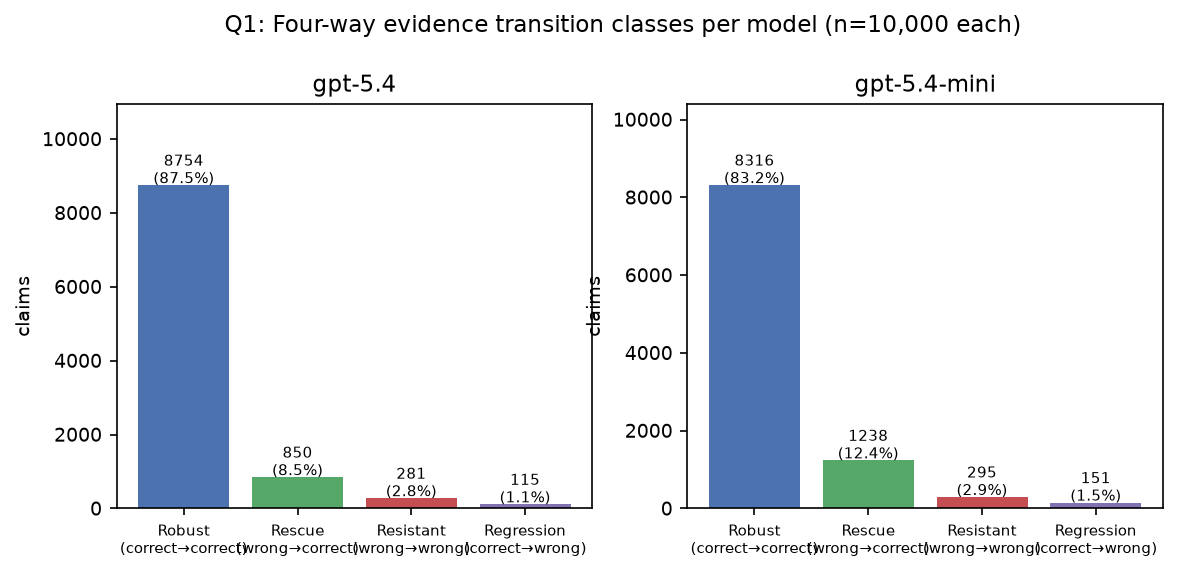
\includegraphics[width=0.92\linewidth]{../analysis_v2/figures/fig1_transition_matrices.png}
\caption{Paired transition matrices for GPT-5.4 and GPT-5.4-mini. Off-diagonal cells are rescues (wrong$\rightarrow$correct) and regressions (correct$\rightarrow$wrong).}
\label{fig:transitions}
\end{figure}

\subsection{Evidence can induce correct-to-wrong regressions}
\label{sec:rq2}
The same paired design produces 115 GPT-5.4 regressions (1.15\%, bootstrap 95\% CI $[0.95,1.36]$) and 151 mini regressions (1.51\%, CI $[1.28,1.75]$).
Rescues are more common: 850 (8.5\%) and 1{,}238 (12.4\%).
Among claim-only errors, evidence corrects 75.2\% (GPT-5.4) and 80.8\% (mini).

Unique-claim counts, not model-observations, are the regression cohort for later adjudication: 226 claims regress for at least one model, 40 for both, and 186 for exactly one (75 GPT-5.4-only, 111 mini-only).
A paired McNemar test on discordant claims finds a modest model difference in regression incidence (115 vs.\ 151, $\chi^2=6.59$, $p=0.010$).
87.3\% of claims share the same transition class across models.
RQ2's answer is therefore: regressions are real, rare relative to 10{,}000 claims, only partly shared, and large enough to study as a structured minority.
These behavioral results come from the original 40{,}000 predictions and are unaffected by the adjudication audit; they are observed outcomes of the original prompts, not evidence of repeat-run stability.

\subsection{Characteristics of evidence-induced regressions}
\label{sec:rq3-nli}
Regressions are not a random slice of the sample.
A local NLI diagnostic (nli-deberta-v3-small) disagrees with the FEVER label on 74.8\% of GPT-5.4 regressions and 76.8\% of mini regressions, against 22.6\% of GPT-5.4 robust successes (Figure~\ref{fig:nli}).
Resistant failures look similar (75.8\%).
A second, architecturally different NLI model reproduces the same ordering.
The 2{,}462 claims flagged as weakly warranted also have lower claim-only GPT-5.4 accuracy (81.0\% vs.\ 88.69\%), so the NLI signal marks hard items rather than a quirk of one evidence-condition model.

\begin{figure}[t]
\centering
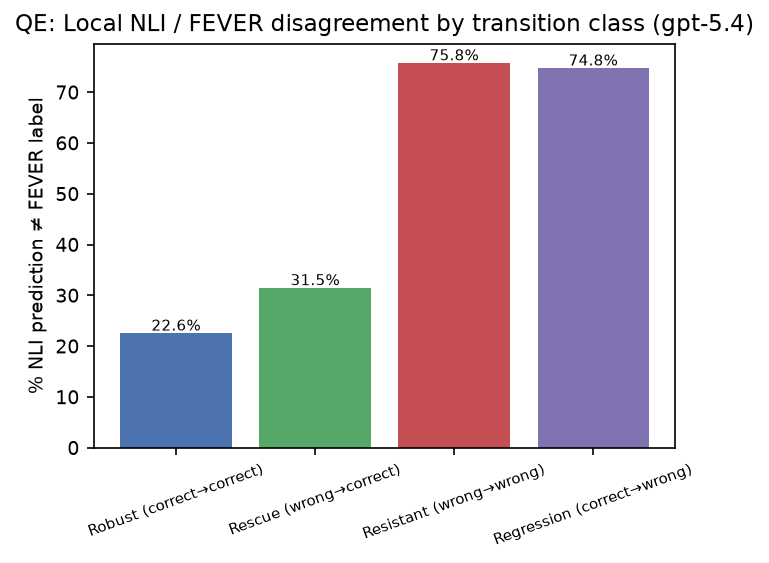
\includegraphics[width=0.88\linewidth]{../analysis_v2/figures/fig6_nli_disagreement.png}
\caption{Local NLI disagreement with the FEVER label by GPT-5.4 transition class. The NLI models are diagnostics, not a relabeling of FEVER.}
\label{fig:nli}
\end{figure}

Label asymmetry is model-dependent.
GPT-5.4 regressions concentrate on Supported claims (88 vs.\ 27 Refuted, $p=1.8\times 10^{-8}$); mini shows no such split (74 vs.\ 77, $p=0.87$).
Surface features (length, overlap, evidence-set size) only weakly separate regressions.
Predictive models that include NLI features do better than surface-only models, but rare-class PR-AUC remains low.
We treat this block as characterization; it does not depend on the adjudication stage that was corrected.

\subsection{Adjudication outcomes on repaired evidence}
\label{sec:rq3-adjudication}
Table~\ref{tab:diagnostic} and Figure~\ref{fig:categories} answer RQ3 for the 226 regressions.
Values in this and the next subsection use the accepted Stage~C outputs; the first-valid sensitivity selection is given where it differs (Section~\ref{sec:correction}).
The largest Grok categories are sentence-only gold agreement (77; 34.1\%, Wilson 95\% CI 28.2--40.5) and final nondecisiveness (71; 31.4\%, 25.7--37.7), whose intervals overlap.
Decisive verdicts that disagree with FEVER form the third group (44; 19.5\%, 14.8--25.1).
Title, structured and additional-evidence gold agreement together cover 29 claims (12.8\%), and five claims follow a nonmonotonic path.
Among regressions with a decisive Stage~C consensus, the Grok verdict agrees with FEVER on 111 of 155 (71.6\%).

\begin{figure}[t]
\centering
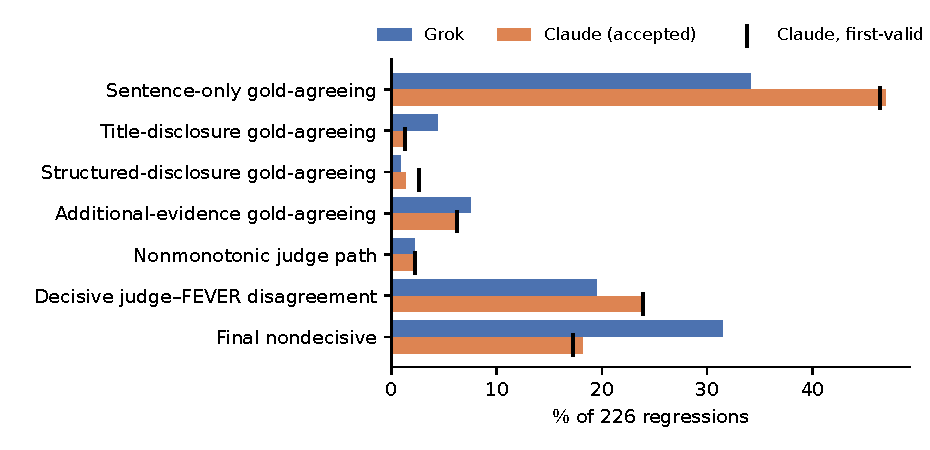
\includegraphics[width=0.95\linewidth]{figures/fig_categories.pdf}
\caption{Adjudication outcome categories for the 226 unique regressions on repaired Stage~C inputs, by adjudicating family. Bars use the accepted outputs; black ticks mark Claude under the first-valid sensitivity selection. Grok values are identical under both selections.}
\label{fig:categories}
\end{figure}

Progressive disclosure changes a minority of verdicts (Table~\ref{tab:stage}, Figure~\ref{fig:stage}).
Titles make 16 of the 103 Stage~A-nondecisive regressions decisive, and Stage~C makes 27 of the 95 Stage~B-nondecisive regressions decisive.
No decisive consensus is reversed by titles or by Stage~C.
Because Stage~C adds alternative sentence text for 41 regressions, Stage~C-associated changes cannot be attributed to representation alone; the 17 additional-evidence cases are separated from the two structure-only cases for that reason.

Shared regressions remain nondecisive more often than model-specific ones (Table~\ref{tab:shared}): 45.0\% versus 28.5\% under Grok (odds ratio 2.05, $p_{\mathrm{BH}}=0.059$).

The RQ3 answer is a mixture of FEVER-agreeing, FEVER-disagreeing and nondecisive outcomes, with no single dominant category under Grok.
These outcomes do not show why GPT changed its answer, and the decisive disagreements are not evidence that FEVER is wrong.

\subsection{Cross-family comparison}
\label{sec:rq4}
The Claude panel judges the same 226 regressions (1{,}130 new Stage~C judgments, paired with its 2{,}260 retained Stage~A/B judgments).
Claude assigns more regressions to sentence-only gold agreement (106, 46.9\%, CI 40.5--53.4; first-valid 105; $+12.8$ and $+12.4$~pp versus Grok, $p_{\mathrm{BH}}\le 2.1\times 10^{-6}$) and fewer to final nondecisiveness (41, 18.1\%, CI 13.7--23.7; first-valid 39; $-13.3$ and $-14.2$~pp, $p_{\mathrm{BH}}\le 9.1\times 10^{-8}$).
Decisive judge--FEVER disagreement is somewhat more common under Claude (54 versus 44; $+4.4$~pp, $p_{\mathrm{BH}}=0.015$).
Among decisive Stage~C consensus verdicts, FEVER agreement is similar across families (Claude 131/185, 70.8\%; Grok 111/155, 71.6\%).

Claude is more decisive at every stage (Table~\ref{tab:stage}, Figure~\ref{fig:stage}): nondecisive rates are 29.2\%, 28.3\% and 18.1\% (first-valid 17.3\%) versus Grok's 45.6\%, 42.0\% and 31.4\%.
Titles resolve 9 of Claude's 66 Stage~A-nondecisive regressions and Stage~C resolves 24 of its 64 Stage~B-nondecisive regressions (first-valid 27).
Title and Stage~C resolution rates do not differ significantly between families, and neither family reverses a decisive consensus.

\begin{figure}[t]
\centering
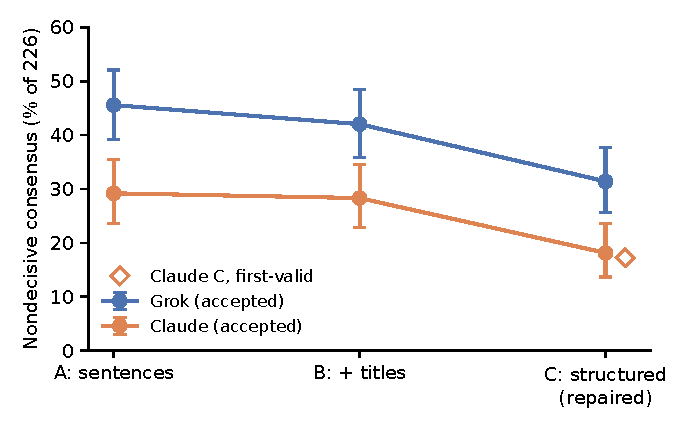
\includegraphics[width=0.62\linewidth]{figures/fig_stage_nondecisive.pdf}
\caption{Nondecisive (Ambiguous or Unresolved) five-judge consensus on the 226 regressions at each disclosure stage, with Wilson 95\% intervals. Stages~A and~B are retained historical judgments on unchanged inputs; Stage~C is new judgments on repaired inputs. The open diamond is Claude Stage~C under the first-valid sensitivity selection.}
\label{fig:stage}
\end{figure}
Under Claude, shared regressions are also more often nondecisive than model-specific ones (35.0\% versus 14.5\%; odds ratio 3.17, $p_{\mathrm{BH}}=0.011$; first-valid 3.47, $p_{\mathrm{BH}}=0.005$).

Exact per-claim category agreement is 172/226 (76.1\%, Wilson 70.1--81.2; $\kappa=0.673$) for the accepted selection and 168/226 (74.3\%, 68.3--79.6; $\kappa=0.651$) for first-valid.
The first-valid figure coincides numerically with the historical 74.3\%, which measured a different, withdrawn taxonomy on defective inputs; the two are not comparable.

\paragraph{Selection sensitivity.}
Substituting the first valid outputs for the accepted ones changes Stage~C consensus for six of the 226 Claude claims and for one of the 1{,}060 Grok claims (a rescue-cohort claim, so no Grok regression result changes).
All 14 cross-family tests and both odds-ratio tests keep their Benjamini--Hochberg decisions, and the only sign change is the non-significant Stage~C resolution difference ($-1.3$ to $0.0$~pp).
Across all 12 combinations of completed runs for the two affected Claude jobs, zero to six claims change consensus relative to the accepted outputs and Claude Stage~C Ambiguous counts range from 37 to 42 of 226.

\subsection{Supporting Stage~A check}
\label{sec:supporting}
GLM-5.3 Stage~A, compared with frozen Cursor Stage~A on 1{,}060 items, yields modal verdict agreement 0.862 and consensus agreement 0.831.
GLM is less ambiguity-conservative (ambiguous/unresolved rate 0.223 vs.\ Cursor 0.291).
This is Stage~A robustness only; Stage~A inputs were unaffected by the audit.

\subsection{What depends on the judge family}
\label{sec:what-replicates}
Common to both families: all categories occur; each disclosure step resolves a minority of the regressions that were nondecisive before it and never reverses a decisive consensus; roughly a fifth to a quarter of regressions end in a decisive verdict opposite to FEVER; decisive verdicts agree with FEVER at similar rates; and shared regressions are more often nondecisive (significant under Claude only).

Family-dependent: absolute nondecisiveness at every stage (13--16~pp lower under Claude), the share of sentence-only gold agreement, and therefore which category is largest.
Per-claim assignment agrees on roughly three claims in four ($\kappa=0.65$--$0.67$).
RQ4's answer is that the qualitative mixture is shared while its proportions are family-dependent.
The design cannot decide whether Claude is better calibrated or more overconfident on thin warrants, because both panels are models scoring the same packets.

\section{Discussion}
\label{sec:discussion}

\subsection{Evidence helps globally but can hurt locally}
The practical headline is not that gold evidence fails.
It succeeds on average, and it rescues far more claim-only errors than it creates.
The scientific headline is that those averages are the wrong unit for reliability engineering.
A 1.15--1.51\% regression rate is small in a 10{,}000-claim table and large if each regression is a previously correct decision that evidence reversed.
Evaluation reports that publish only condition-wise accuracy will miss that reversal.

\subsection{What adjudication can and cannot say about regressions}
For roughly a third (Grok) to nearly half (Claude) of the 226 regressions, a blinded panel reaches the FEVER label from the evidence sentences alone and keeps it as titles and structured evidence are added.
On those items the designated evidence appears adequate to an independent reader while GPT moved away from the correct label after receiving it.
That pattern is compatible with an evidence-utilization failure and connects to work showing that models can ignore, mishandle, or be distracted by supplied context \citep{longpre-etal-2021-entity,shi2023distracted,wan-etal-2024-evidence}.
It does not establish that explanation: the original runs stored labels only, and the adjudicator is a different model reading the evidence in a different prompt.
A further fifth to quarter of regressions end in a decisive verdict opposite to FEVER, and a sixth (Claude) to nearly a third (Grok) end nondecisive.
In neither case does a decisive GPT answer after evidence show that GPT failed to use evidence supporting the FEVER answer.
These observations therefore do not establish the prevalence or cause of GPT evidence-utilization failures.

\subsection{Nondecisiveness and disagreement with FEVER}
Final nondecisiveness is common in both families, which is expected given prior evidence that sufficiency and ambiguity are first-class problems in fact verification \citep{atanasova-etal-2022-fact,glockner-etal-2024-ambifc}.
We do not interpret nondecisive outcomes or decisive judge--FEVER disagreements as FEVER annotation errors; inspected rationales show substantive conflicts (for example, a date or scope mismatch between claim and evidence), but judge rationales are observations, not labels.
Shared regressions, which both GPT models got wrong after evidence, are more often nondecisive under both families, although the Grok difference is not significant after correction.

\subsection{Disclosure and representation}
Titles and structured evidence change a minority of verdicts and never reverse a decisive consensus.
Stage~C adds alternative sentence text for some claims, so its effect mixes added information with changed representation.
Separating the two would require a structure-only arm that shows the chosen evidence set without alternatives; we did not run one.
We therefore make no claim about the size or portability of a pure representation effect.

\subsection{Judge-family dependence as measurement uncertainty}
The Claude-versus-Grok difference is a result, not a defect to be explained away.
LLM-as-judge work already shows that evaluators have family-specific biases and are not drop-in substitutes \citep{zheng2023judging,liu-etal-2023-g,chen-etal-2024-humans,huang-etal-2025-empirical}.
Here the same packets, rubric, and taxonomy produce a 13--16~pp difference in nondecisiveness at every stage and disagreement on about one regression in four.
Category shares are therefore properties of an adjudicating family as much as of the claims; two instruments do not define an uncertainty interval for a latent prevalence, and we report both rather than a single estimate.

\subsection{Implications for evidence-grounded LLM evaluation}
Four implications follow.
First, paired no-evidence versus gold-evidence evaluation should be standard whenever a benchmark supplies designated evidence; otherwise regressions are invisible.
Second, automated diagnostic categories need a second judge family before their shares are treated as stable, and decisiveness should be reported separately from agreement with the benchmark label.
Third, residual nondecisiveness should remain a first-class output of adjudication rather than being forced into Supported/Refuted.
Fourth, adjudication inputs deserve the same verification as model inputs: a field-extraction error silently corrupted the structured stage of our original adjudication.
% COAUTHOR REVIEW: the historical draft named 58 claim-level disagreements; the corrected count is 54 (accepted) or 58 (first-valid).
Human review of the 54--58 claim-level Grok--Claude category disagreements would be the natural next measurement, not another automated family.

\section{Limitations}
\label{sec:limitations}

All adjudication is automated silver labeling.
Grok, GLM, and Claude judgments are not expert human annotation and do not create a new gold standard.
Within-family agreement overstates how much independent human raters would agree, because the five judges are isolated contexts of one locked model.

Category shares are judge-family-sensitive.
We report both complete panels and refuse a single point estimate.

FEVER labels remain the behavioral gold standard.
NLI disagreement and judge--FEVER disagreement mark candidate ambiguity; they do not prove an annotation is wrong.

The study is binary Supported/Refuted FEVER, 2017-era Wikipedia claims, and designated gold evidence rather than retrieved open-web context.
\texttt{NOT ENOUGH INFO} is excluded by design.

Both evaluated systems are GPT-5.4 variants.
Transition concordance can reflect family-correlated errors.

Progressive disclosure locates where a judge panel's verdict changes.
It does not observe GPT-internal causal mechanisms, and the original GPT runs stored labels only.

The historical adjudication's Stage~C packets displayed corrupted sentence text, and its taxonomy conflated disagreement with FEVER with evidence utilization.
The repaired Stage~C and the descriptive taxonomy were specified post hoc, after the historical results and defects were inspected; the correction protocol is not a preregistration and the taxonomy awaits coauthor review.
Stage~C adds alternative evidence text for some claims, so Stage~C-associated changes are not a pure representation manipulation.

Consensus paths combine retained historical Stage~A/B judgments with new Stage~C judgments.
The historical protocol specified a fresh context per judge, batch and stage, but raw historical session transcripts were not available to verify runtime isolation independently.

Execution of the Stage~C re-judging deviated from its frozen protocol: six jobs exceeded the three-attempt cap after quota and usage-limit failures; concurrent runners left collision records whose sessions are unknown; one collision record was deleted during execution and survives only in a session transcript; and in two Claude jobs a later output was accepted although earlier finished runs had produced schema-valid outputs.
The protocol's primary analysis is therefore incomplete, and the diagnostic results come from a separately labeled analysis whose input selections were specified after the outputs were inspected.
Selection sensitivity is bounded (at most six Claude claims change), but the analysis cannot be presented as the protocol's pre-specified result.

The protocol's follow-up panels were not run: a newly selected residual Claude panel, a Stage~C resolver, and an optional fixed historical residual panel.
The Claude panel covers the 226 regressions, not the 1{,}060-item judged cohort, and GLM is Stage~A only.
Historical execution events in the original Claude panel (a quarantined path-leak rerun, a usage-limit pause, and a duplicate-batch tie-break) affect only its retained Stage~A/B judgments and are documented in Appendix~\ref{app:historical-deviations}.

\section{Conclusion}
\label{sec:conclusion}

Designated gold evidence improves GPT-5.4 and GPT-5.4-mini fact verification in aggregate and still induces 226 unique correct-to-wrong regressions.
These behavioral results are unchanged by the adjudication audit.
Re-adjudicated on repaired structured evidence by two model families, the regressions form a mixture of FEVER-agreeing, FEVER-disagreeing and nondecisive panel outcomes; disclosure of titles and structured evidence resolves a minority of them and never reverses a decisive verdict.
The historical three-way failure-mode shares and their cross-family ordering are withdrawn: category proportions depend on the adjudicating family, and the adjudication does not identify why GPT changed its answers.
Because the re-judging deviated from its frozen protocol, the corrected diagnostic figures are a dated post-judgment analysis, reported with their selection sensitivity and pending coauthor review.


\section*{Data and code}
The behavioral record is tag \texttt{evidex-artifact-v1} at commit \texttt{29102c3}; its headline verifiers and test suites are unchanged.
The evidence audit, repaired Stage~C packets, frozen correction protocol (2026-09-27), all execution records including failed attempts, and the post-judgment deviation analysis are on branch \texttt{codex/methodology-correction-v2}.
Project code is MIT-licensed; FEVER and Wikipedia-derived files are third-party material.

\bibliography{../paper/references}

\appendix
\section{Execution deviations in the corrected Stage~C}
\label{app:correction-deviations}

The correction protocol was frozen on 2026-09-27 with no judgment outputs present.
It required 70 jobs (55 Grok on 1{,}060 claims; 15 Claude on 226 claims; 6{,}430 judgments), at most three attempts per job, acceptance of the first schema-valid response, and a unique session per attempt.
All 70 jobs delivered schema-valid outputs; every attempt, including failures, is archived byte-exact.

Provider quota exhaustion and an account usage limit caused repeated failed attempts.
With operator authorization, six jobs (two Grok, four Claude) were retried beyond three attempts; in five of them the accepted output was the first schema-valid output, and in the sixth (\texttt{p02\_C\_j2\_b03}) it was the first that could be checkpointed.
Two runner processes operated concurrently for part of the execution and wrote 13 collision records whose session is unknown; we keep those records as \texttt{unknown} rather than infer whether a run was launched.
In two Claude jobs (\texttt{p02\_C\_j2\_b02}, \texttt{p02\_C\_j2\_b03}), earlier runs finished with schema-valid outputs that were never checkpointed because collision records occupied their slots; a later output was accepted.
During one of those jobs a collision record was deleted so the running attempt could checkpoint; the deletion survives only in a session transcript.
In one Grok job (\texttt{p01\_C\_j5\_b09}) a run wrote a complete schema-valid output and then ended with a provider error; the next run was accepted.

The frozen validator therefore reports incomplete provenance, and no judgment freeze or protocol result set exists.
The post-judgment deviation analysis applies the frozen analysis and taxonomy code unchanged to (i)~the 70 accepted outputs and (ii)~the first finished schema-valid output for each Claude job.
It also enumerates all 12 combinations of completed runs for the two affected Claude jobs (0--6 claims change Stage~C consensus; Claude Ambiguous 37--42), and treats the error-ending Grok output as a separate sensitivity (one consensus label changes, on a non-regression claim).
These selections were specified after the outputs were inspected.

\section{Historical execution events in the Claude full panel}
\label{app:historical-deviations}

The historical Claude full panel reused the locked model \texttt{claude-opus-5-thinking-high}, the shared rubric, and the blinded Stage~A/B/C evidence files; its Stage~A/B judgments are retained in this draft and its historical Stage~C judgments are not used.
During the first Stage~A batch-01 wave, judge-facing file paths included the panel directory name and therefore the cohort-selection criterion.
Before inspecting the affected judgments, the five delivered files (5$\times$77 $= 385$ valid records) were quarantined, judge I/O moved to a neutral directory, and that batch rerun under the unchanged model, rubric, and evidence packets.
No quarantined verdict was read.
Stage~B was interrupted by a usage limit after 601 of 1{,}130 judgments; work resumed on the same Claude slug and already-valid judgments were kept.
Recovery overlap caused three judge-batches to be produced twice; a first-ingested-wins rule, applied without reading either copy's labels, retained one file per $(\mathrm{stage},\mathrm{judge},\mathrm{item})$.

\section{Withdrawn historical diagnostic results}
\label{app:historical}

The following results appeared in the historical draft (\texttt{paper/}, preserved unchanged).
They were computed with the legacy three-way taxonomy on Stage~C packets that displayed corrupted sentence text, and they are withdrawn as estimates.
They are listed only so readers can trace the correction.
\begin{itemize}
\item Grok three-way split of the 226 regressions: 50.0\% evidence-utilization failure, 11.9\% representation-sensitive, 38.1\% residual ambiguity (113/27/86). Of the 113 legacy utilization cases, 36 had a decisive Stage~C verdict opposite to FEVER.
\item Claude three-way split: 65.9\% / 5.3\% / 28.8\% (149/12/65); 46 of the 149 legacy utilization cases disagreed with FEVER at Stage~C.
\item ``Utilization failure is largest in both panels'' and the claimed replication of the category ordering; the 50--66\% range for utilization failure.
\item Legacy taxonomy agreement 74.3\% (168/226), $\kappa=0.537$, and the four-item representation-sensitive overlap.
\item Historical Stage~C nondecisive rates (Grok 38.1\%, Claude 28.8\%) and the Stage~C-dependent McNemar test.
\item The historical Claude residual test (134/231, 58.0\%, persistently ambiguous), whose inputs and residual selection both depended on defective Stage~C.
\end{itemize}
Historical figures of the category split, taxonomy confusion, Stage~C ambiguity and Grok resolution flow are not reproduced in this draft.

\section{Denominator checklist}
\label{app:denoms}

\begin{tabular}{lr}
\toprule
Quantity & $n$ \\
\midrule
FEVER claims in the paired experiment & 10{,}000 \\
GPT predictions & 40{,}000 \\
Diagnostic-cohort claims constructed & 1{,}061 \\
Judged diagnostic-cohort items & 1{,}060 \\
Unique regressions & 226 \\
New Stage~C judgments, Grok (1{,}060 $\times$ 5) & 5{,}300 \\
New Stage~C judgments, Claude (226 $\times$ 5) & 1{,}130 \\
Required correction jobs delivered & 70 \\
Retained historical Claude Stage~A/B judgments & 2{,}260 \\
Optional historical-residual judgments (not run) & 1{,}155 \\
\bottomrule
\end{tabular}


\end{document}
